\documentclass[12pt, a4paper]{article}

\usepackage{amsmath}
\usepackage{array}
\usepackage{amsmath}
\usepackage[portuguese]{babel}
\usepackage{chngpage}
\usepackage{float}
\usepackage[a4paper, margin=2cm]{geometry}
\usepackage{graphicx}
\usepackage{hyperref}
\usepackage{listings}
\usepackage{setspace}
\usepackage{xcolor}

\lstdefinestyle{codestyle}{
    commentstyle=\color{teal},
    keywordstyle=\color{blue},
    numberstyle=\ttfamily\color{gray},
    stringstyle=\color{red},
    basicstyle=\ttfamily\footnotesize,
    breakatwhitespace=false,
    breaklines=false,
    keepspaces=true,
    numbers=none,
    showspaces=false,
    showstringspaces=false,
    showtabs=false,
    tabsize=4
}
\lstset{style=codestyle}

\title{\Huge \textbf{Computação Gráfica \\ \Large Trabalho Prático -- Fase II}}
\date{30 de março 2025}
\author{Grupo 3}

\begin{document}

\begin{center}
    
\includegraphics[width=0.25\textwidth]{res/cover/EE-C.eps}
\end{center}

\chardef\_=`_
\onehalfspacing
\setlength{\parskip}{\baselineskip}
\setlength{\parindent}{0pt}
\def\arraystretch{1.5}

{\let\newpage\relax\maketitle}
\maketitle
\thispagestyle{empty}

\vspace*{\fill}

\begin{adjustwidth}{-2cm}{-2cm} % These values only need to be large enough to center the table
    \begin{center}
        \begin{tabular}{>{\centering}p{0.25\textwidth}
                        >{\centering}p{0.25\textwidth}
                        >{\centering}p{0.25\textwidth}
                        >{\centering\arraybackslash}p{0.25\textwidth}}
            
\includegraphics[width=3.5cm]{res/cover/A104437.png} &
            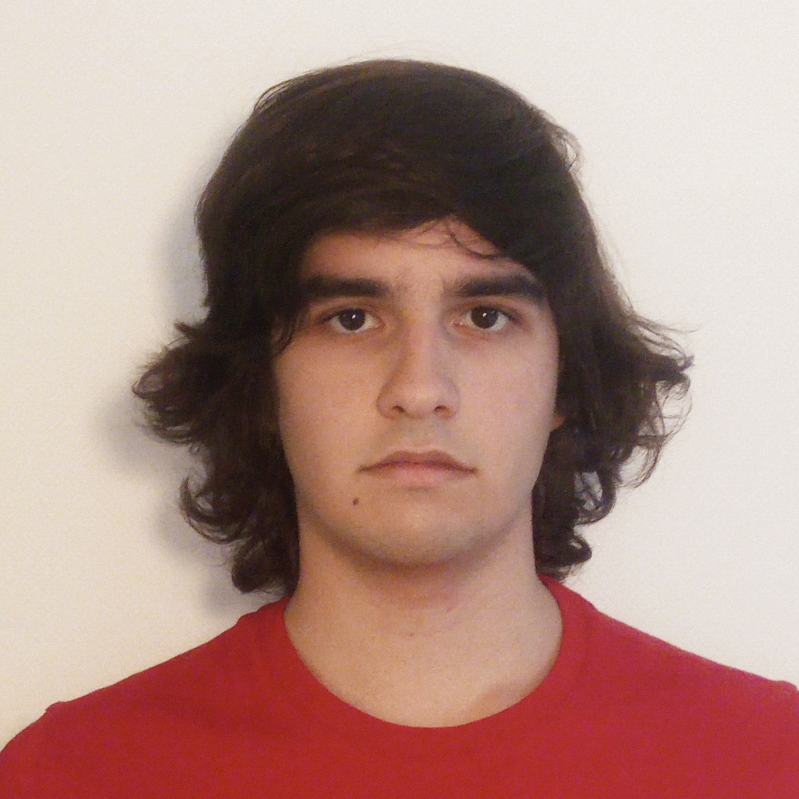
\includegraphics[width=3.5cm]{res/cover/A104348.png} &
            
\includegraphics[width=3.5cm]{res/cover/A90817.png} &
            
\includegraphics[width=3.5cm]{res/cover/A104179.png} \\

            Ana Oliveira & Humberto Gomes & Mariana Cristino & Sara Lopes \\
            A104437      & A104348        & A90817           & A104179
        \end{tabular}
    \end{center}
\end{adjustwidth}

\pagebreak

\begin{abstract}
    \textbf{\color{red} TODO - resumo}
\end{abstract}

\section{Transformações}

\textbf{\color{red} TODO - transformações}

\section{Modelo estático do sistema solar}

\textbf{\color{red} TODO - sistema solar}

\section{Extras}

Nesta fase, fizemos vários extras:
\begin{itemize}
    \item Geração de Möbius Strip;
    \item \color{red} TODO
    \item \color{red} TODO
    \item \color{red} TODO
\end{itemize}
\subsection{\emph{Möbius Strip}}

Para gerar um \emph{möbius strip} é necessário ter um raio, uma largura, o número de slices,
o número de stacks e o ficheiro onde se irá colocar os vértices e as faces desta figura.
Um \emph{möbius strip} clássico possui uma torção (uma meia volta), mas para tornar a geração
da figura mais interessante, é possível incluir o parâmetro de número de torções (meias voltas
dadas), permitindo variações no modelo.
\begin{verbatim}
    ./generator mobiusStrip <radius> <width> <twist> <slices> <stacks> <file>
\end{verbatim}

Matematicamente, as coordenadas de um ponto do \emph{möbius strip} são definidas do seguinte modo:

$$x = (radius + \theta \times \frac{width}{2} \times \cos (\frac{twist}{2} \times \phi)) \times
\cos (\phi)$$
$$y = \theta \times \frac{width}{2} \times \sin (\frac{twist}{2} \times \phi)$$
$$z = (radius + \theta \times \frac{width}{2} \times \cos (\frac{twist}{2} \times \phi)) \times
\sin (\phi)$$

$$\phi \in \left [ 0, 2 \pi \right [$$
$$\theta \in \left [ -1, 1 \right ]$$

radius, width e twist são os parâmetros dados para a geração do \emph{möbius strip}, o raio, a
largura e o número de torções, respetivamente.

$\phi$ varia entre 0 e $2 \pi$ e $\theta$ varia entre -1 e 1.

Para gerar uma nuvem de pontos uniformemente distribuídos percorremos a faixa pelo seu comprimento
(pelas fatias ou slices) e pela sua largura (pelos segmentos ou stacks).

$$
\phi_i = i \cdot \frac{2\pi}{N_\text{slices}}
\hspace{1cm}
i \in \left \lbrace 0, 1, \ldots, N_\text{slices} \right \rbrace
$$

$$
\theta_j = j \cdot \frac{2}{N_\text{stacks}} -1
\hspace{1cm}
j \in \left \lbrace 0, 1, \ldots, N_\text{stacks} \right \rbrace
$$

Assim, o \emph{möbius strip} é gerado iterando sobre os valores inteiros possíveis de i e j,
o que dá origem à nuvem de pontos desejada.

Após a geração dos vértices, estes são agrupados nos triângulos que compõem a superfície do
\emph{möbius strip}.
Para isso, considera-se um vértice de referência, como P1, juntamente com o vértice
adjacente na mesma fatia (P3) e os dois vértices correspondentes na fatia seguinte (P2 e P4),
e geram-se quatro faces triangulares: duas faces de um lado e outras duas faces do outro lado
do quadrilátero formado por estes quatro vértices. Este processo repete-se para todos os vértices
onde é aplicável, garantindo que cada célula quadrangular é subdividida em quatro triângulos.
A figura seguinte ilustra esse processo, mostrando a organização dos triângulos resultantes:

\begin{figure}[H]
    \centering
    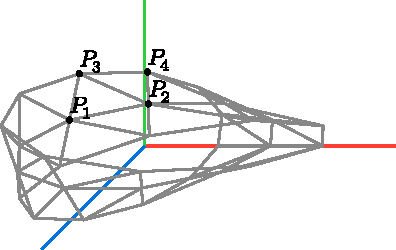
\includegraphics[width=0.35\textwidth]{res/phase2/figures/MobiusStrip.pdf}
    \caption{Faces do \emph{möbius strip} geradas numa iteração.}
\end{figure}

Como \emph{möbius strip} é uma faixa, então desenha-se os dois lados da faixa. É por
isto que geramos faces com os mesmos pontos mas com ordenações dos pontos diferentes:
geramos tanto as faces de um lado da faixa como as faces do outro lado.
Para os quatro pontos apresentados acima, os triângulos gerados são os seguintes:

$$
T_1 = (P_1, P_2, P_3)
\hspace{1cm}
T_2 = (P_2, P_1, P_3)
\hspace{1cm}
T_3 = (P_3, P_2, P_4)
\hspace{1cm}
T_4 = (P_2, P_3, P_4)
$$

Com o \texttt{generator} foi criado um modelo do \emph{möbius strip}. Com esse modelo
foi criada uma cena que foi renderizada pela \texttt{engine} da seguinte forma:

\begin{figure}[H]
    \centering
    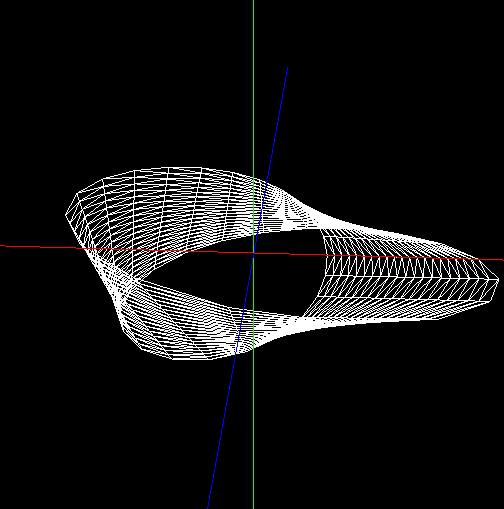
\includegraphics[width=0.35\textwidth]{res/phase2/figures/MobiusStrip.png}
    \caption{\emph{Möbius Strip}}
\end{figure}

\textbf{\color{red} TODO - extras continuação}

\section{Resultados obtidos}

\textbf{\color{red} TODO - resultados}

\section{Conclusão e Trabalho Futuro}

\textbf{\color{red} TODO - conclusão}

\begingroup
\section{Bibliografia}
\renewcommand{\section}[2]{}

\begin{thebibliography}{9}
    \bibitem{möbius strip}
        "Möbius Strip."{} Wolfram MathWorld. Accessed: Mar. 25, 2025. [Online.] Available:
        \url{https://mathworld.wolfram.com/MoebiusStrip.html}
\end{thebibliography}
\endgroup

\end{document}
